% Options for packages loaded elsewhere
\PassOptionsToPackage{unicode}{hyperref}
\PassOptionsToPackage{hyphens}{url}
%
\documentclass[
]{article}
\usepackage{amsmath,amssymb}
\usepackage{lmodern}
\usepackage{iftex}
\ifPDFTeX
  \usepackage[T1]{fontenc}
  \usepackage[utf8]{inputenc}
  \usepackage{textcomp} % provide euro and other symbols
\else % if luatex or xetex
  \usepackage{unicode-math}
  \defaultfontfeatures{Scale=MatchLowercase}
  \defaultfontfeatures[\rmfamily]{Ligatures=TeX,Scale=1}
\fi
% Use upquote if available, for straight quotes in verbatim environments
\IfFileExists{upquote.sty}{\usepackage{upquote}}{}
\IfFileExists{microtype.sty}{% use microtype if available
  \usepackage[]{microtype}
  \UseMicrotypeSet[protrusion]{basicmath} % disable protrusion for tt fonts
}{}
\makeatletter
\@ifundefined{KOMAClassName}{% if non-KOMA class
  \IfFileExists{parskip.sty}{%
    \usepackage{parskip}
  }{% else
    \setlength{\parindent}{0pt}
    \setlength{\parskip}{6pt plus 2pt minus 1pt}}
}{% if KOMA class
  \KOMAoptions{parskip=half}}
\makeatother
\usepackage{xcolor}
\usepackage[margin=1in]{geometry}
\usepackage{graphicx}
\makeatletter
\def\maxwidth{\ifdim\Gin@nat@width>\linewidth\linewidth\else\Gin@nat@width\fi}
\def\maxheight{\ifdim\Gin@nat@height>\textheight\textheight\else\Gin@nat@height\fi}
\makeatother
% Scale images if necessary, so that they will not overflow the page
% margins by default, and it is still possible to overwrite the defaults
% using explicit options in \includegraphics[width, height, ...]{}
\setkeys{Gin}{width=\maxwidth,height=\maxheight,keepaspectratio}
% Set default figure placement to htbp
\makeatletter
\def\fps@figure{htbp}
\makeatother
\setlength{\emergencystretch}{3em} % prevent overfull lines
\providecommand{\tightlist}{%
  \setlength{\itemsep}{0pt}\setlength{\parskip}{0pt}}
\setcounter{secnumdepth}{-\maxdimen} % remove section numbering
\usepackage{booktabs}
\usepackage{longtable}
\usepackage{array}
\usepackage{multirow}
\usepackage{wrapfig}
\usepackage{float}
\usepackage{colortbl}
\usepackage{pdflscape}
\usepackage{tabu}
\usepackage{threeparttable}
\usepackage{threeparttablex}
\usepackage[normalem]{ulem}
\usepackage{makecell}
\usepackage{xcolor}
\ifLuaTeX
  \usepackage{selnolig}  % disable illegal ligatures
\fi
\IfFileExists{bookmark.sty}{\usepackage{bookmark}}{\usepackage{hyperref}}
\IfFileExists{xurl.sty}{\usepackage{xurl}}{} % add URL line breaks if available
\urlstyle{same} % disable monospaced font for URLs
\hypersetup{
  pdftitle={Mercado de Trabalho no Setor Portuário brasileiro e maranhense},
  pdfauthor={Observatório Portuário},
  hidelinks,
  pdfcreator={LaTeX via pandoc}}

\title{Mercado de Trabalho no Setor Portuário brasileiro e maranhense}
\author{Observatório Portuário}
\date{}

\begin{document}
\maketitle

{
\setcounter{tocdepth}{2}
\tableofcontents
}
\hypertarget{introduuxe7uxe3o}{%
\section{Introdução}\label{introduuxe7uxe3o}}

O setor portuário brasileiro impacta direta e indiretamente os destinos
e a economia do país.

O Observatório Portuário apresenta neste relatório uma síntese da
evolução do Trabalho Portuário e aquaviário no Brasil e no Maranhão.

Trata-se de um setor abrangente e com atividades diversas como
instalações portuárias, embarcações mercantes, de passageiros, pesca,
atividades em plataformas marítimas e de repação naval.

Como se trata de uma ampla gama de atividades, o relatório estará
organizado em duas seções com focos direcionados: a primeira com um
panorama abarcado pelo Trabalho Portuário e aquaviário e a segunda com
um recorte específico sobre a operação e gestão portuária.

\hypertarget{metodologia}{%
\subsection{Metodologia}\label{metodologia}}

Os dados apresentados neste relatório são originários da Relação Anual
de Informações Sociais (RAIS).

A RAIS é um registro administrativo que as organizações públicas e
privadas são obrigadas a enviar ao Ministério da Economia anualmente.
Seus dados, assim, abarcam estabelecimentos formais e permitem
identificar o estoque de vínculos formais de emprego (estatutários e
celetistas).

Este relatório apresenta os dados em uma perspectiva longitudinal:
apresenta os dados de 2010 a 2020.

O recorte dos dados sobre o trabalho portuário e aquaviário foi
realizado a partir da Classificação Nacional de Atividades Econômicas
(CNAE).

A CNAE é a classificação oficialmente adotada pelo Sistema Estatístico
Nacional e pelos órgãos federais gestores de registros administrativos e
está organizada em ordem decrescente de agregação das informações:
Seções, Divisões, Grupos, Classes e Subclasses.

A partir dessa divisão é possível mapear as atividades com trabalho
portuário e aquaviário e, especificamente, de operações e gestão
portuária.

Na tabela estão detalhadas as informações da CNAE utilizadas:

\begin{table}

\caption{\label{tab:tabela1}<center>Subclasses da Classificação Nacional de Atividades Econômicas 2.0 usadas <br> Seção H: Transporte, Armazenagem e Correio</center>}
\centering
\begin{tabular}[t]{>{}lllll}
\toprule
Seção & Divisão & Grupo & Classe & Subclasse\\
\midrule
 &  &  &  & Administração da infra-estrutura portuária\\
\cmidrule{5-5}
 & \multirow[t]{-2}{*}{\raggedright\arraybackslash ARMAZENAMENTO E ATIVIDADES AUXILIARES DOS TRANSPORTES} & \multirow[t]{-2}{*}{\raggedright\arraybackslash Atividades auxiliares dos transportes aquaviários} & \multirow[t]{-2}{*}{\raggedright\arraybackslash Gestão de portos e terminais} & Operações de terminais\\
\cmidrule{2-5}
 &  &  &  & Navegação de apoio marítimo\\
\cmidrule{5-5}
 &  & \multirow[t]{-2}{*}{\raggedright\arraybackslash Navegação de apoio} & \multirow[t]{-2}{*}{\raggedright\arraybackslash Navegação de apoio} & Navegação de apoio portuário\\
\cmidrule{3-5}
 &  &  &  & Transporte por navegação de travessia, intermunicipal\\
\cmidrule{5-5}
 &  &  & \multirow[t]{-2}{*}{\raggedright\arraybackslash Transporte por navegação de travessia} & Transporte por navegação de travessia, municipal\\
\cmidrule{4-5}
 &  &  &  & Outros transportes aquaviários não especificados anteriormente\\
\cmidrule{5-5}
 &  & \multirow[t]{-4}{*}{\raggedright\arraybackslash Outros transportes aquaviários} & \multirow[t]{-2}{*}{\raggedright\arraybackslash Transportes aquaviários não especificados anteriormente} & Transporte aquaviário para passeios turísticos\\
\cmidrule{3-5}
 &  &  &  & Transporte marítimo de cabotagem - Carga\\
\cmidrule{5-5}
 &  & \multirow[t]{-2}{*}{\raggedright\arraybackslash Transporte marítimo de cabotagem e longo curso} & \multirow[t]{-2}{*}{\raggedright\arraybackslash Transporte marítimo de cabotagem} & Transporte marítimo de cabotagem - passageiros\\
\cmidrule{3-5}
 &  &  &  & Transporte por navegação interior de carga, intermunicipal, interestadual e internacional, exceto travessia\\
\cmidrule{5-5}
 &  &  & \multirow[t]{-2}{*}{\raggedright\arraybackslash Transporte por navegação interior de carga} & Transporte por navegação interior de carga, municipal, exceto travessia\\
\cmidrule{4-5}
 &  &  &  & Transporte por navegação interior de passageiros em linhas regulares, intermunicipal, interestadual e internacional, exceto travessia\\
\cmidrule{5-5}
\multirow[t]{-14}{*}{\raggedright\arraybackslash \textbf{H}} & \multirow[t]{-12}{*}{\raggedright\arraybackslash TRANSPORTE AQUAVIÁRIO} & \multirow[t]{-4}{*}{\raggedright\arraybackslash Transporte por navegação interior} & \multirow[t]{-2}{*}{\raggedright\arraybackslash Transporte por navegação interior de passageiros em linhas regulares} & Transporte por navegação interior de passageiros em linhas regulares, municipal, exceto travessia\\
\bottomrule
\multicolumn{5}{l}{\rule{0pt}{1em}\textit{Note: } makecell[l]{Observatório Portuário \Dados: IBGE - CNAE}}\\
\end{tabular}
\end{table}

\hypertarget{panorama-do-trabalho-no-setor-portuuxe1rio-e-aquaviuxe1rio-no-brasil}{%
\section{Panorama do trabalho no setor portuário e aquaviário no
Brasil}\label{panorama-do-trabalho-no-setor-portuuxe1rio-e-aquaviuxe1rio-no-brasil}}

Foram 76.350 vínculos registrados no setor portuário e aquaviário no
Brasil em 2020, de acordo com os dados da Relação Anual de Informações
Sociais (RAIS).

O número apresenta um decréscimo em relação aos anos anteriores,
sobretudo em relação ano de 2018, quando quase 80 mil vínculos foram
registrados. Considerando a tendência de queda do número de vínculos
identificada a partir de 2014, reitera-se a associação entre desempenho
das atividades econômicas do país e sua influência no estoque de
empregos do setor.

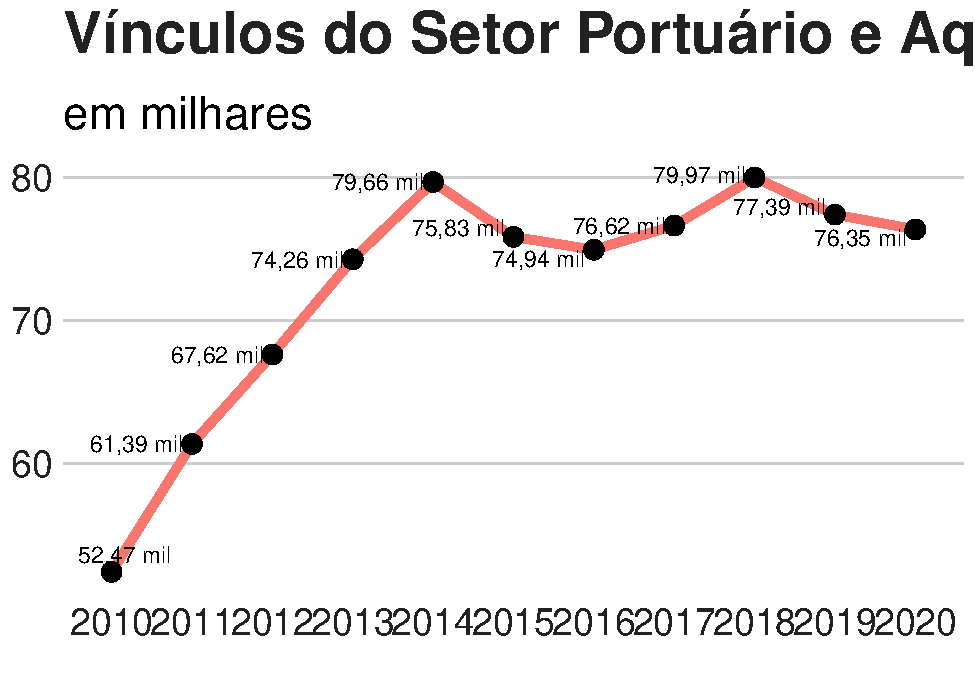
\includegraphics{mercado_trabalho_files/figure-latex/g_secao-1.pdf}

Ao analisar os dados por setor de atividade, verifica-se redução do
número de vínculos no grupo de profissionais atuantes nos (Divisão,
conforme nomenclatura da CNAE) \textbf{Transportes aquaviários},
conforme se verifica no gráfico, com uma redução de 44.420 mil vínculos
em 2013 para 37.910 mil em 2020, com uma redução de 6.510 vínculos.

Por outro lado, nota-se que o grupo de atividades agrupadas como
\textbf{Armazenamento e Atividades Auxiliares dos Transportes}
apresentou um comportamento crescente no período, superando em 2020 o
número de vínculos no \textbf{Transporte aquaviário}.

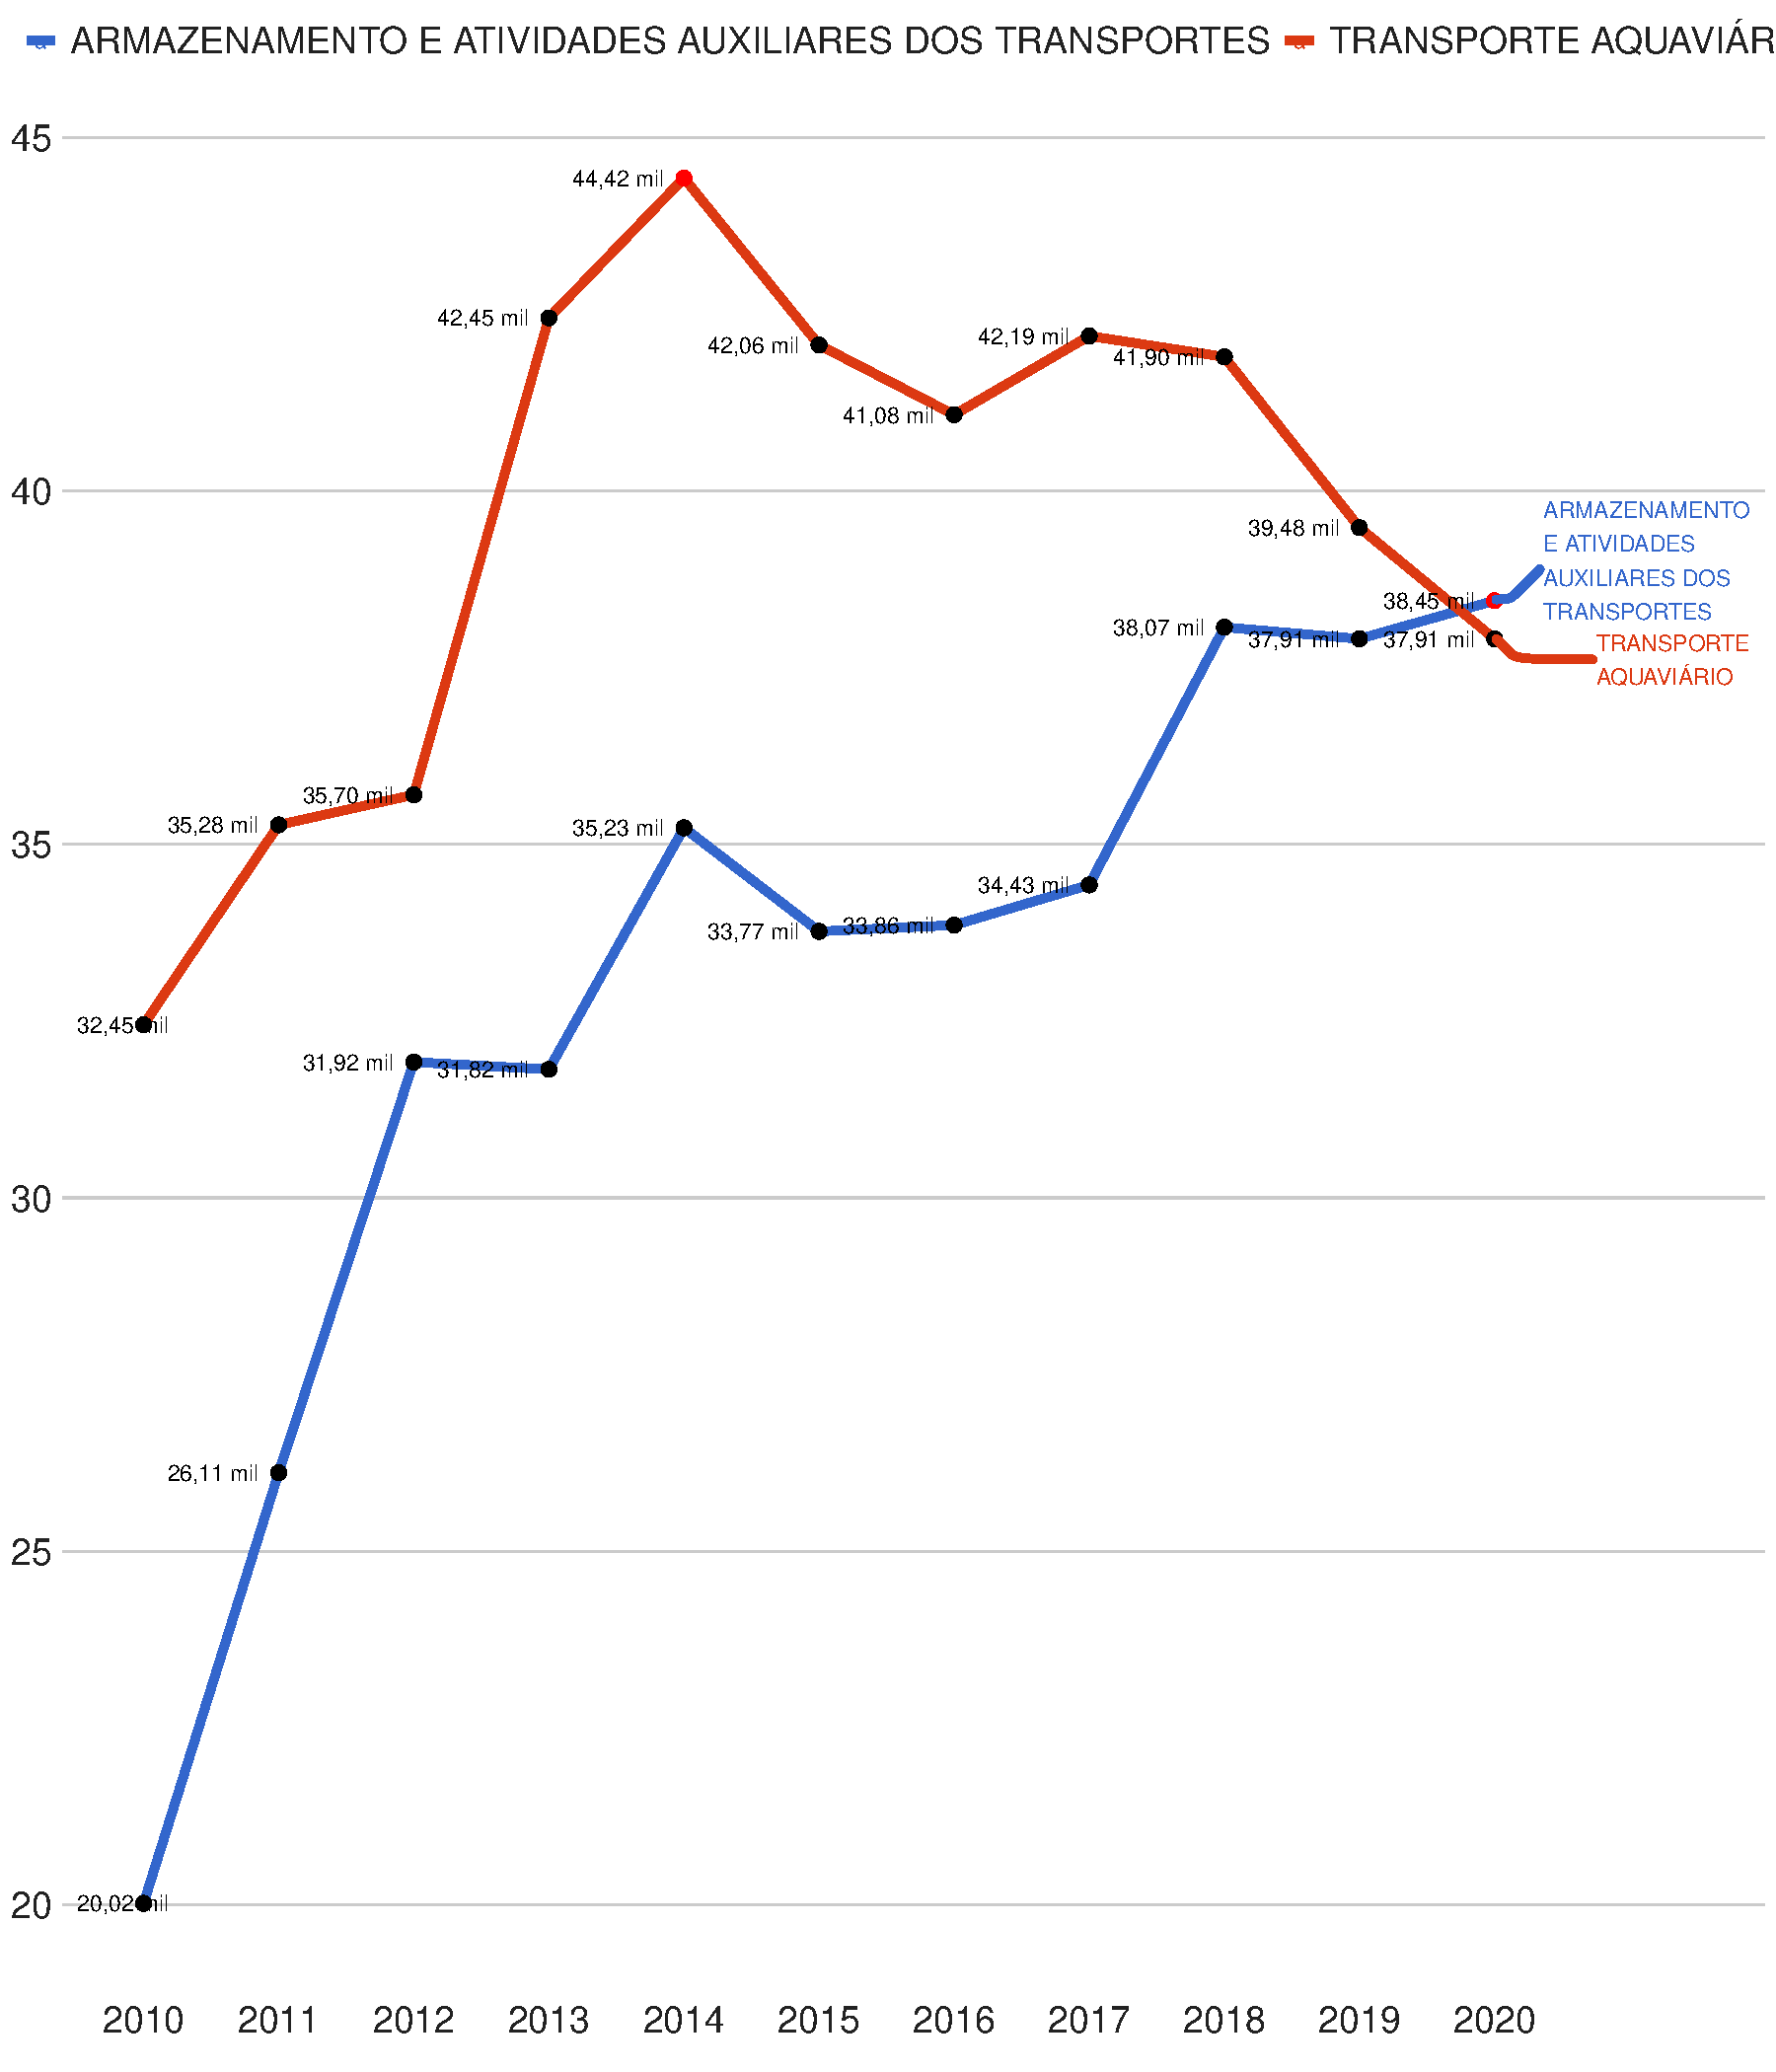
\includegraphics{mercado_trabalho_files/figure-latex/g_divisao-1.pdf}

Ao analisar os grupos de atividades com maiores vínculos, verifica-se o
destaque das atividades de \textbf{Armazenamento e Atividades Auxiliares
dos Transportes}, que compreende, de acordo com a CNAE, atividades
relacionadas

\begin{quote}
{[}\ldots{]} com a movimentação e o armazenamento de cargas, antes ou
depois de seu transporte, ou entre segmentos de transporte de distintas
modalidades, as atividades auxiliares das diversas modalidades de
transporte envolvendo a operação da infraestrutura de suporte nas
rodovias, ferrovias, aeroportos, portos, pontes túneis, etc. e as
atividades de agenciamento de transporte. Esta divisão compreende também
as atividades relacionadas à organização do transporte de carga.
\end{quote}

Destaque também deve ser dado para o número de vínculos em
\textbf{Navegação de Apoio}, que abarca atividades como:

\begin{itemize}
\item
  o transporte de mercadorias e pessoas para suprimento e apoio a navios
  e a plataformas de pesquisas e exploração de minerais e
  hidrocarbonetos;
\item
  a navegação realizada para apoio logístico a navios e a plataformas de
  exploração de minerais e hidrocarbonetos transporte;
\item
  a navegação realizada nos portos e terminais aquaviários, para
  atendimento a embarcações e instalações portuárias;
\item
  os serviços de reboque realizado por empresas de apoio marítimo;
\item
  os serviços de socorro e salvamento realizado por empresas de apoio
  portuário.
\end{itemize}

\hfill\break

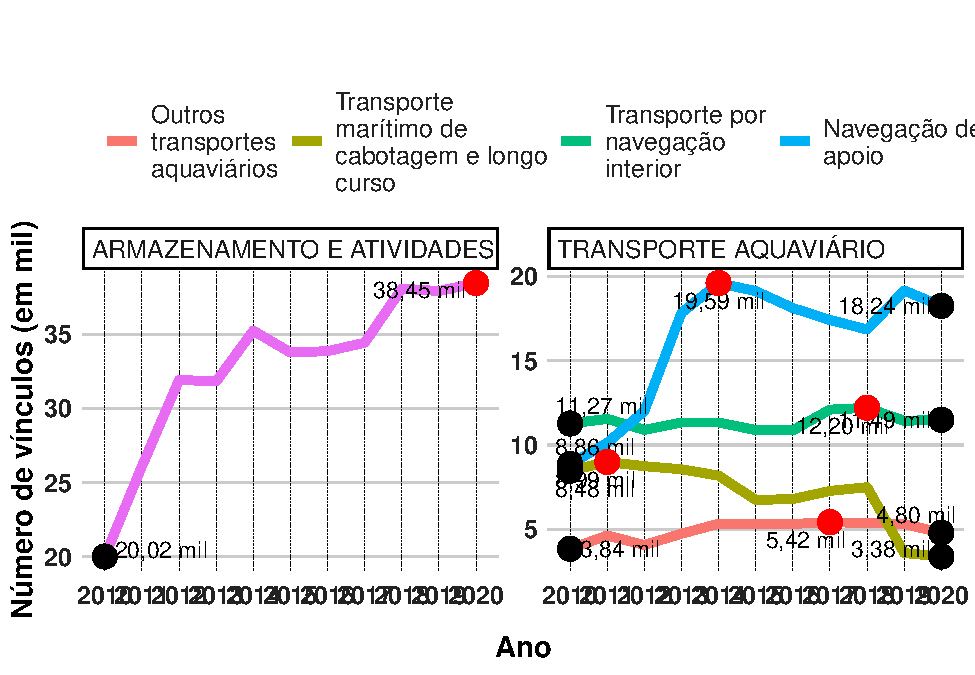
\includegraphics{mercado_trabalho_files/figure-latex/g_grupo-1.pdf}

Observa-se que o grupo de \textbf{Transporte por Navegação Interior}
compreende atividades como \emph{o transporte de carga municipal, por
rios, canais, lagos, lagoas, baias e outras vias de navegação interior,
exceto travessia} e \emph{o fretamento de embarcações com tripulação},
mas não inclui \emph{a operação e gestão de terminais de carga}.

Além disso, a queda do número de vínculos em \textbf{Transporte Marítimo
de Cabotagem e Longo Curso} foi bastante acentuada, saindo de quase 9
mil vínculos em 2010 para menos de 4 mil em 2020.

Ao detalhar as informações, verifica-se que houve acentuado aumento de
vínculos no Brasil nas \textbf{Operações Portuárias}, saltando de 14.760
vínculos para XXX, enquanto houve uma redução na \textbf{Administração
da Infra-Estrutura Portuária}, que em 2010 apresentava pouco mais de 5
mil vínculos e apresentava apenas 3 mil em 2020.

\textbf{Continuar a descrição e melhorar a leitura do gráfico}

\hypertarget{section}{%
\subparagraph{}\label{section}}

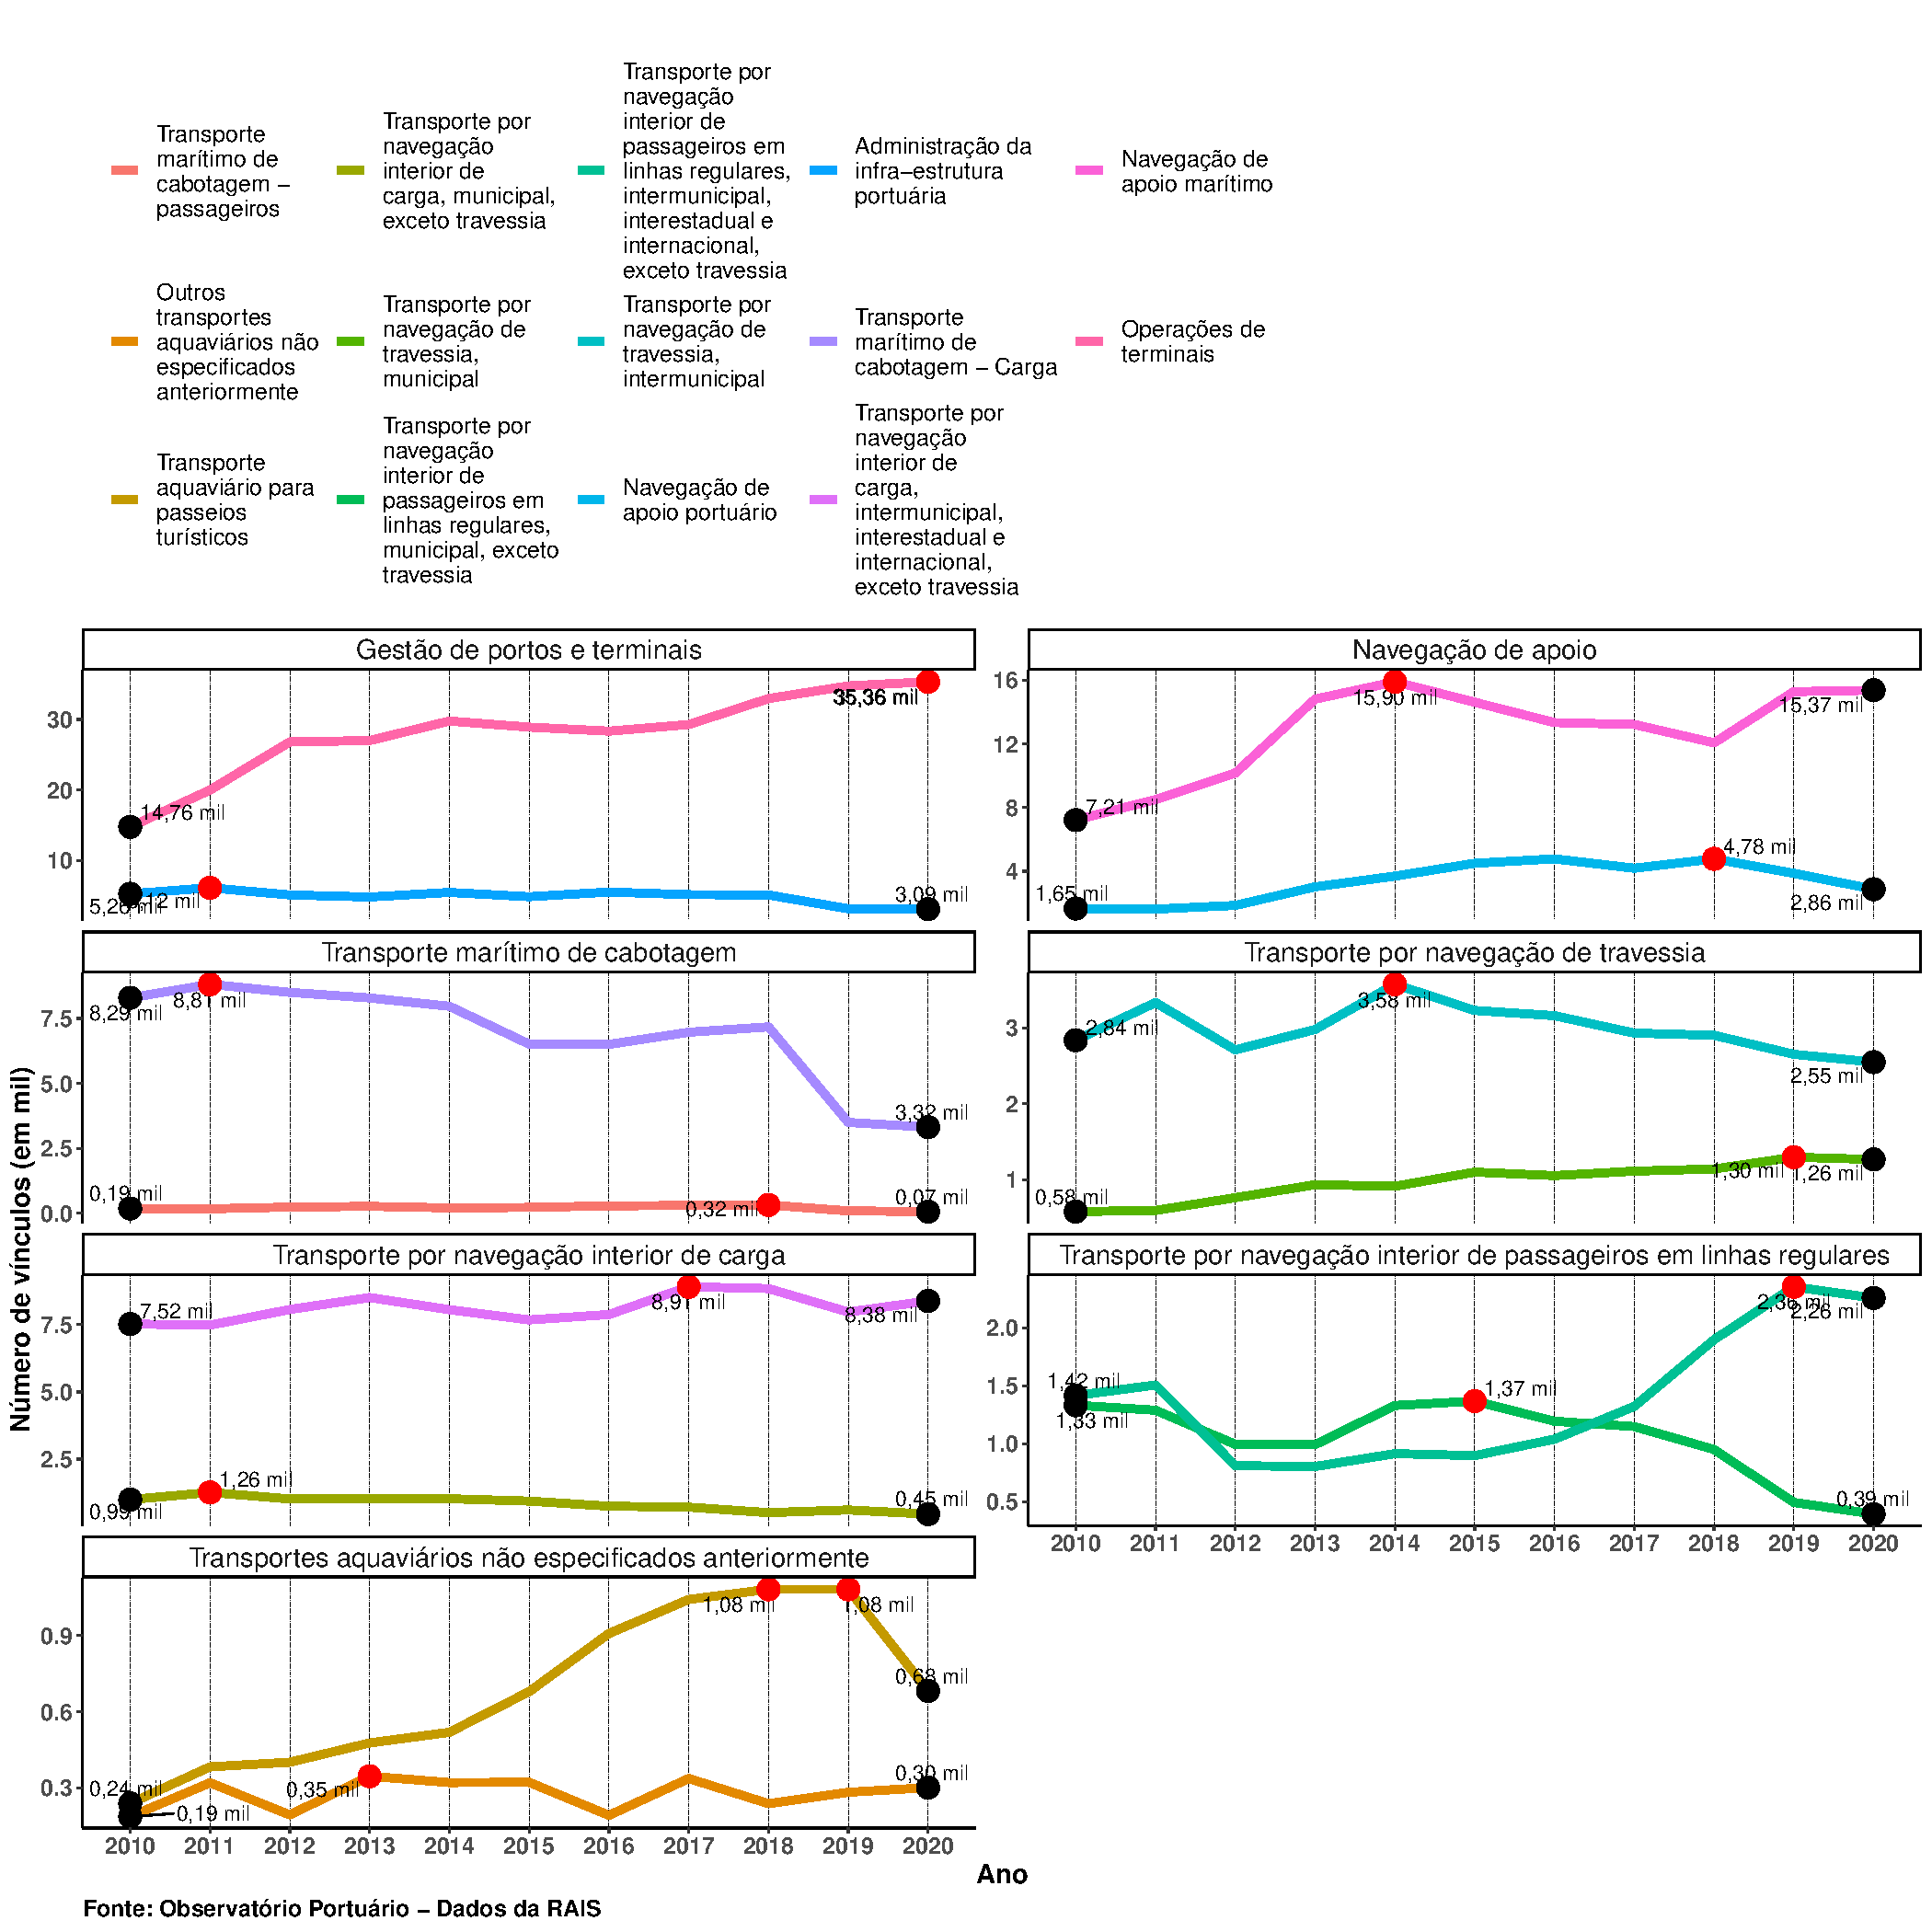
\includegraphics{mercado_trabalho_files/figure-latex/funcao2-1.pdf}

\hypertarget{perfil-do-trabalhador-portuuxe1rio-e-aquaviuxe1rio}{%
\section{Perfil do Trabalhador Portuário e
Aquaviário}\label{perfil-do-trabalhador-portuuxe1rio-e-aquaviuxe1rio}}

\hypertarget{escolaridade-do-trabalhador-portuuxe1rio-e-aquaviuxe1rio}{%
\subsubsection{Escolaridade do Trabalhador Portuário e
aquaviário}\label{escolaridade-do-trabalhador-portuuxe1rio-e-aquaviuxe1rio}}

Ao analisar o perfil dos trabalhadores por sexo, observa-se que a
participação masculina é destacada. Em 2020, do total de 76.317
vínculos, 65.735 eram homens, sendo apenas 10.582 mulheres (13,87\%).

Apesar da baixa participação feminina no setor, observa-se que
apresentam maior escolaridade: 44,5\% têm curso superior, contra 17,7\%
dos homens com a mesma escolaridade. De forma agregada, observa-se o
aumento da escolarização entre 2010 e 2020, apesar do número de
profissionais com pós-graduação ainda ser baixo.

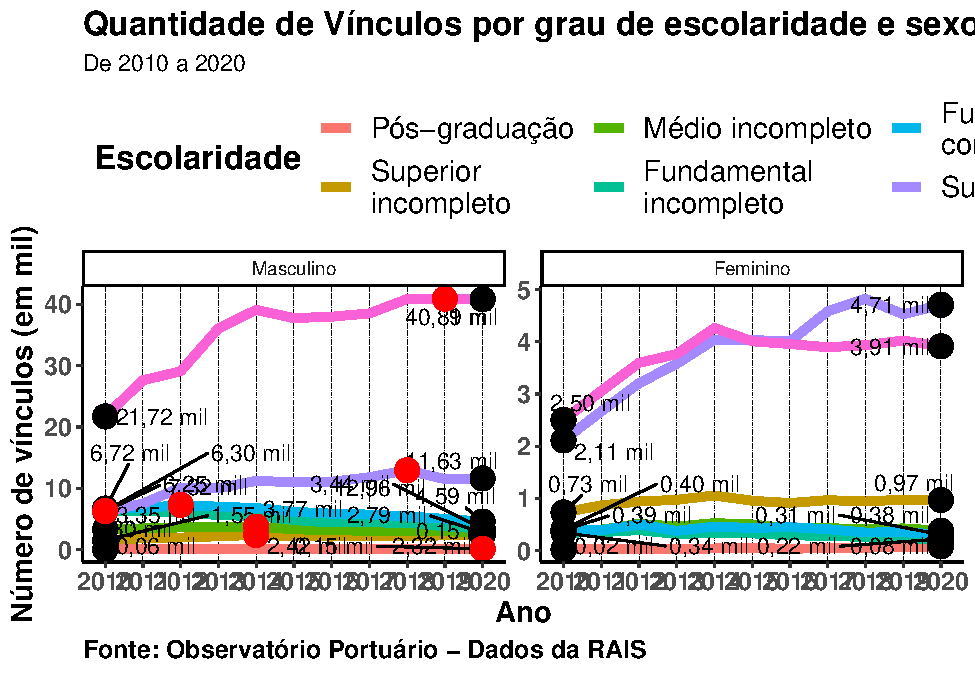
\includegraphics{mercado_trabalho_files/figure-latex/g_operacao_escol_sexo-1.pdf}

\hypertarget{rauxe7a-ou-cor-do-trabalhador-portuuxe1rio-e-aquaviuxe1rio}{%
\subsubsection{Raça ou cor do Trabalhador Portuário e
aquaviário}\label{rauxe7a-ou-cor-do-trabalhador-portuuxe1rio-e-aquaviuxe1rio}}

Como há uma discrepância da quantidade de vínculos das categorias de
\textbf{raça ou cor} quando comparadas por \textbf{sexo}, optou-se pela
\textbf{escala logarítmica} no lugar da escala aritimética (escala
habitual nos gráficos) para representar os dados quantidade de vínculos
(\textbf{eixo y}) , pois a logarítmica permite, no caso do gráfico
abaixo, uma visualização das tendências das quantidades de vínculos por
cada raça ou cor ao longo dos anos analisados.

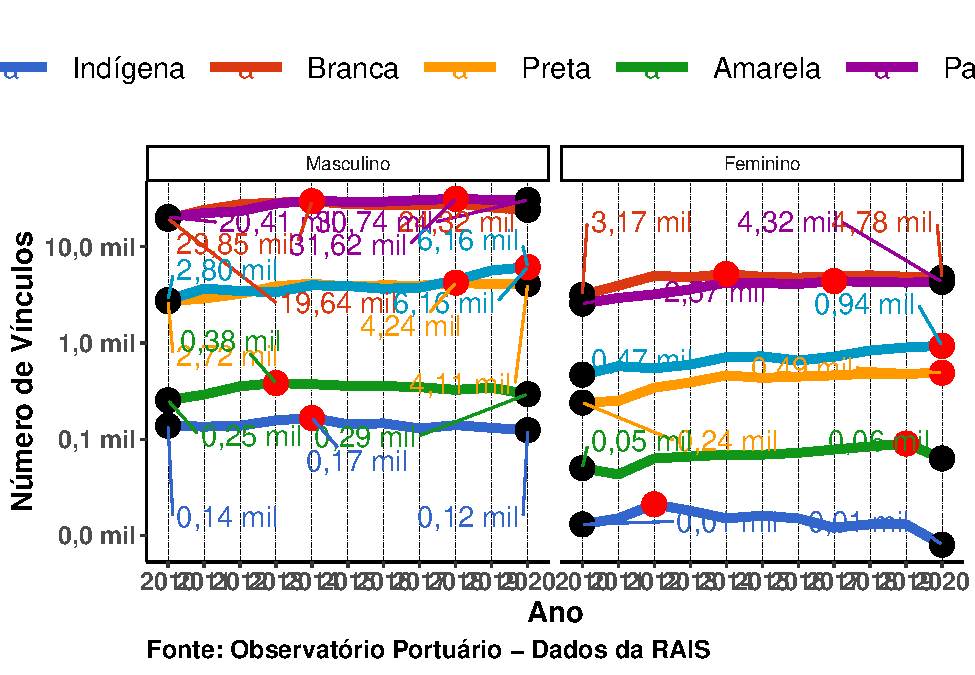
\includegraphics{mercado_trabalho_files/figure-latex/g_operacao_raca_sexo-1.pdf}

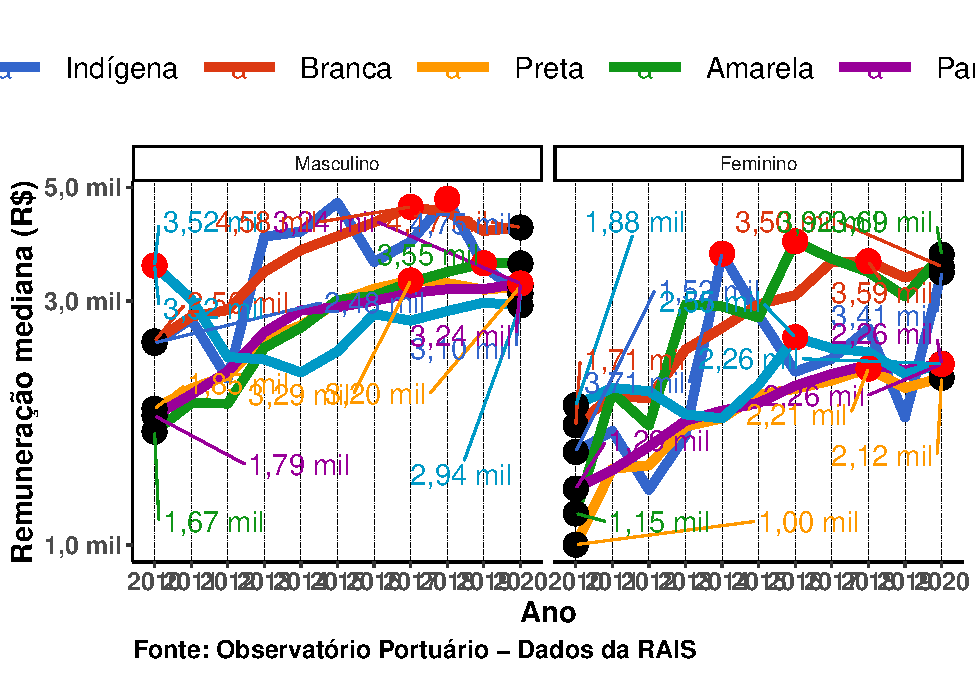
\includegraphics{mercado_trabalho_files/figure-latex/g_operacao_remuneracao _mediana_raca_sexo-1.pdf}

\hypertarget{ocupauxe7uxf5es-dos-trabalhadores-portuuxe1rios-e-aquaviuxe1rios}{%
\subsection{Ocupações dos Trabalhadores Portuários e
Aquaviários}\label{ocupauxe7uxf5es-dos-trabalhadores-portuuxe1rios-e-aquaviuxe1rios}}

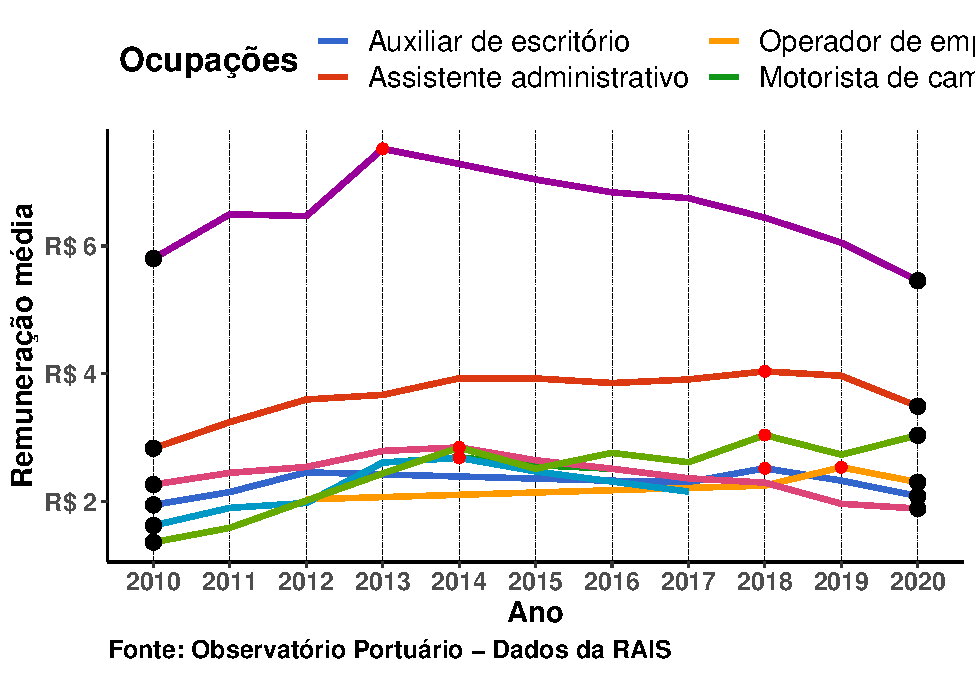
\includegraphics{mercado_trabalho_files/figure-latex/g_operacao_ocupacao-1.pdf}

\hypertarget{remunerauxe7uxe3o-muxe9dia-dos-trabalhadores-nos-estados}{%
\subsection{Remuneração Média dos Trabalhadores nos
Estados}\label{remunerauxe7uxe3o-muxe9dia-dos-trabalhadores-nos-estados}}

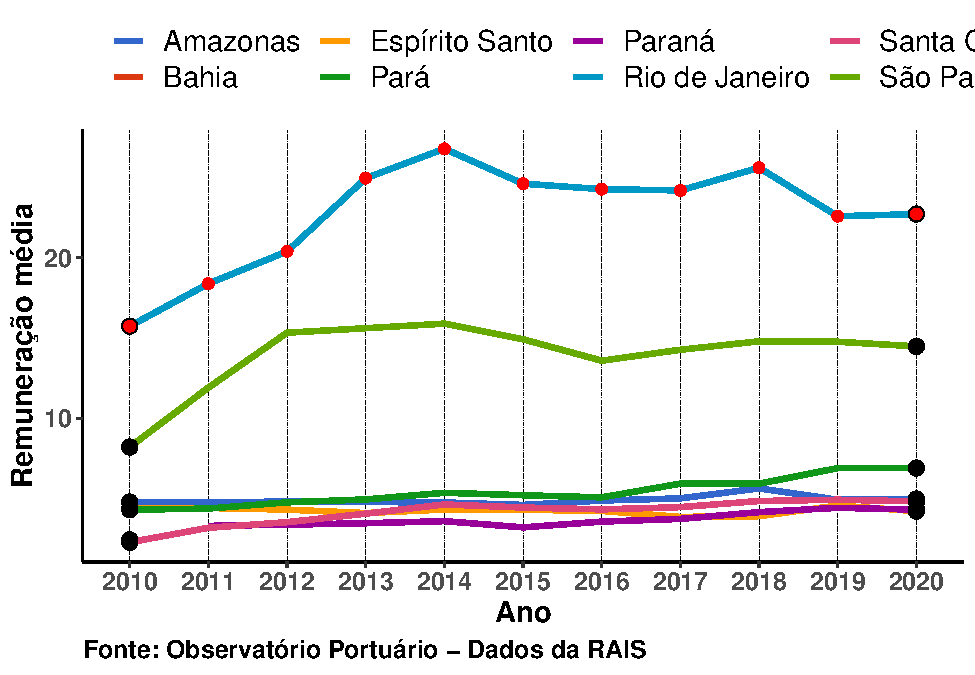
\includegraphics{mercado_trabalho_files/figure-latex/g_operacao_estado-1.pdf}

\hypertarget{remunerauxe7uxe3o-muxe9dia-dos-trabalhadores-nos-municuxedpios}{%
\subsection{Remuneração Média dos Trabalhadores nos
municípios}\label{remunerauxe7uxe3o-muxe9dia-dos-trabalhadores-nos-municuxedpios}}

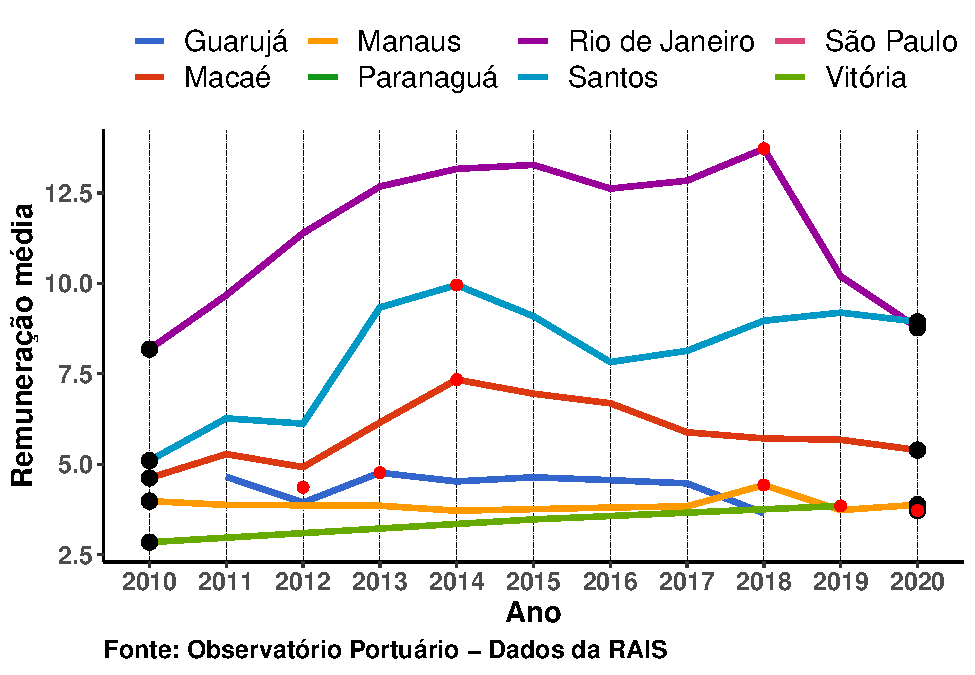
\includegraphics{mercado_trabalho_files/figure-latex/g_operacao_municipio-1.pdf}

\hypertarget{trabalhadores-da-gestuxe3o-e-operauxe7uxe3o-portuuxe1ria}{%
\section{Trabalhadores da Gestão e Operação
Portuária}\label{trabalhadores-da-gestuxe3o-e-operauxe7uxe3o-portuuxe1ria}}

O Brasil apresentou 796.506 vínculos de trabalho para a subclasse
\textbf{Operações de Terminais}. São Paulo foi o estado com a maior
quantidade de vínculos, ao todo foram 15.742, 18.393, 20.403, 22.594,
22.731, 24.203, 24.281, 24.624, 24.967, 25.617, 26.800 vínculos no
estado. Rio de Janeiro, segundo estado com a maior quantidade de
vículos, possuía cerca de 6, 6, 6, 6, 6, 6, 7, 7, 7, 7, 8, 8, 8, 19. O
estado do Maranhão possuía 1.299, 1.357, 1.472, 1.478, 1.546, 1.855,
1.856, 1.890, 1.924, 1.963, 2.016 vínculos.

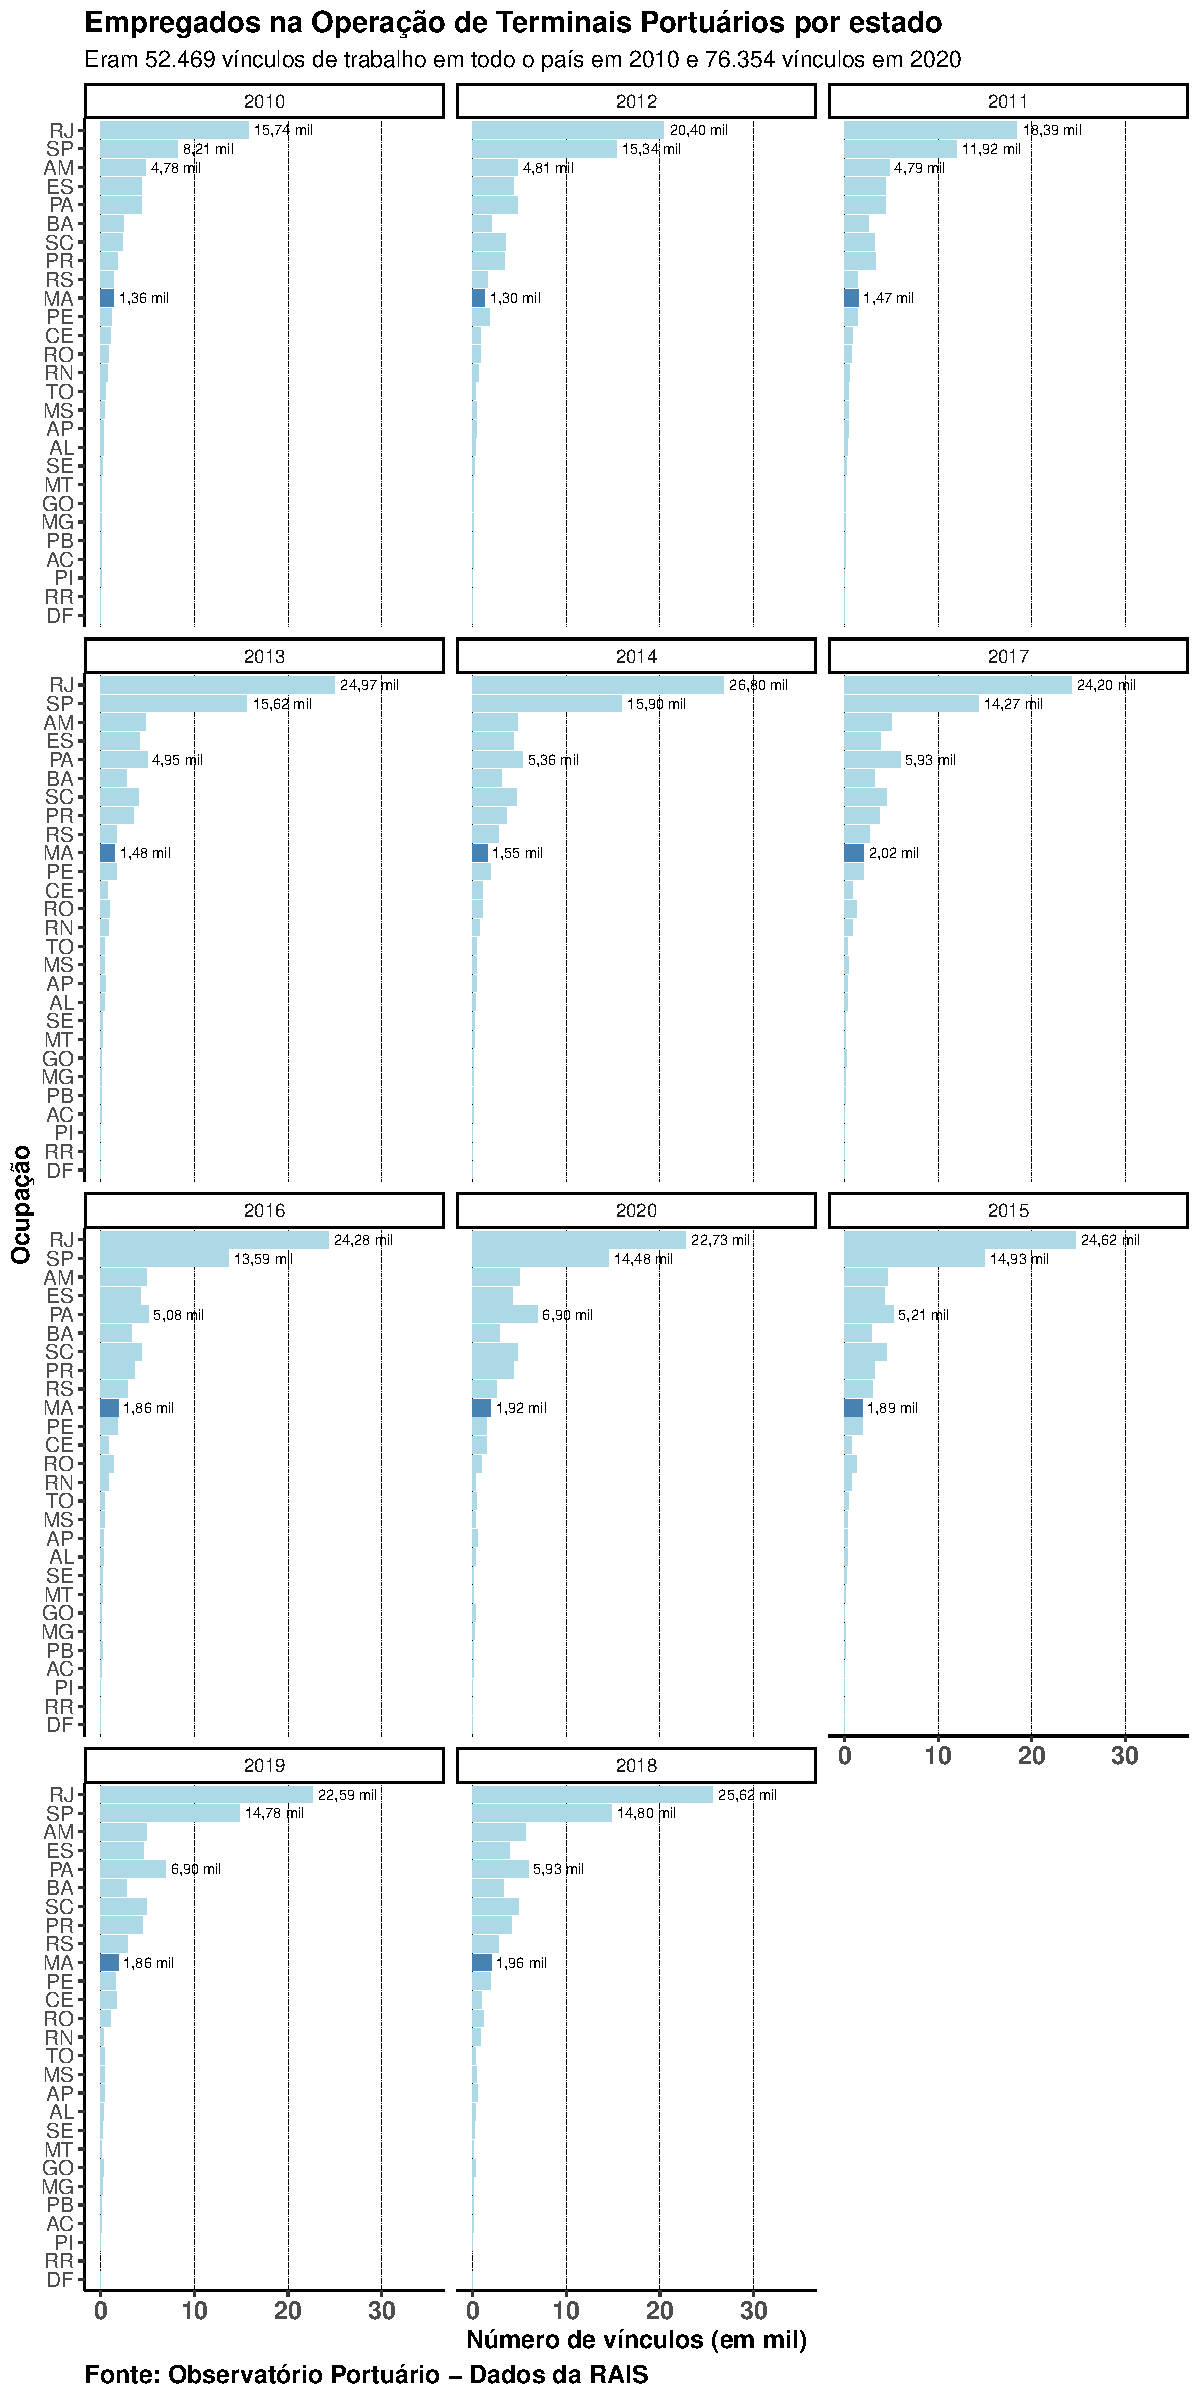
\includegraphics{mercado_trabalho_files/figure-latex/g_operacao_uf-1.pdf}

\hypertarget{panorama-do-trabalho-no-setor-portuuxe1rio-e-aquaviuxe1rio-no-maranhuxe3o}{%
\section{Panorama do trabalho no setor portuário e aquaviário no
Maranhão}\label{panorama-do-trabalho-no-setor-portuuxe1rio-e-aquaviuxe1rio-no-maranhuxe3o}}

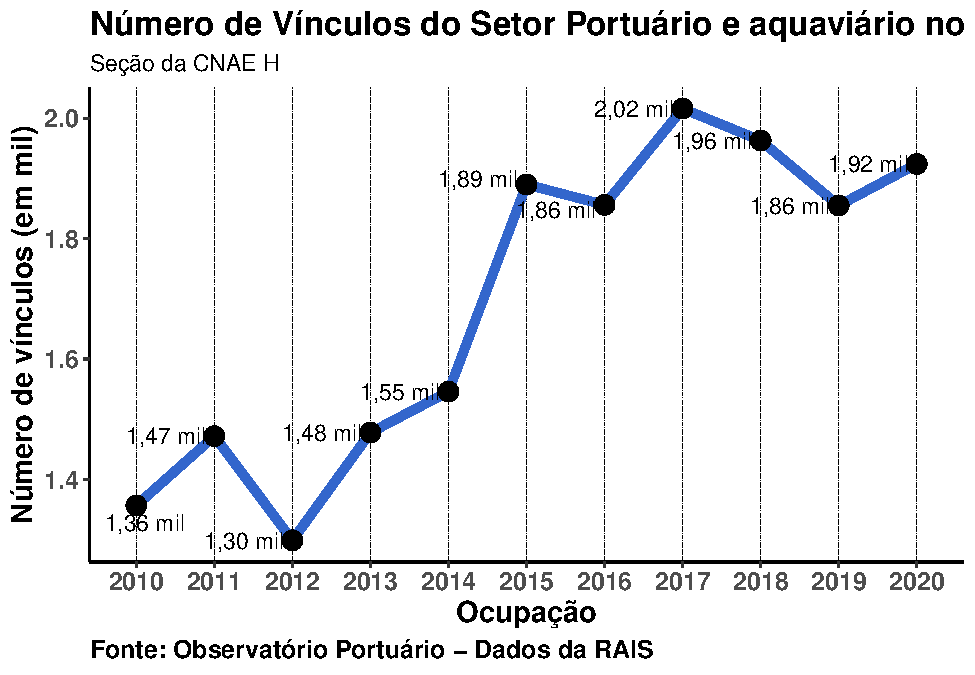
\includegraphics{mercado_trabalho_files/figure-latex/g_secao_ma-1.pdf}

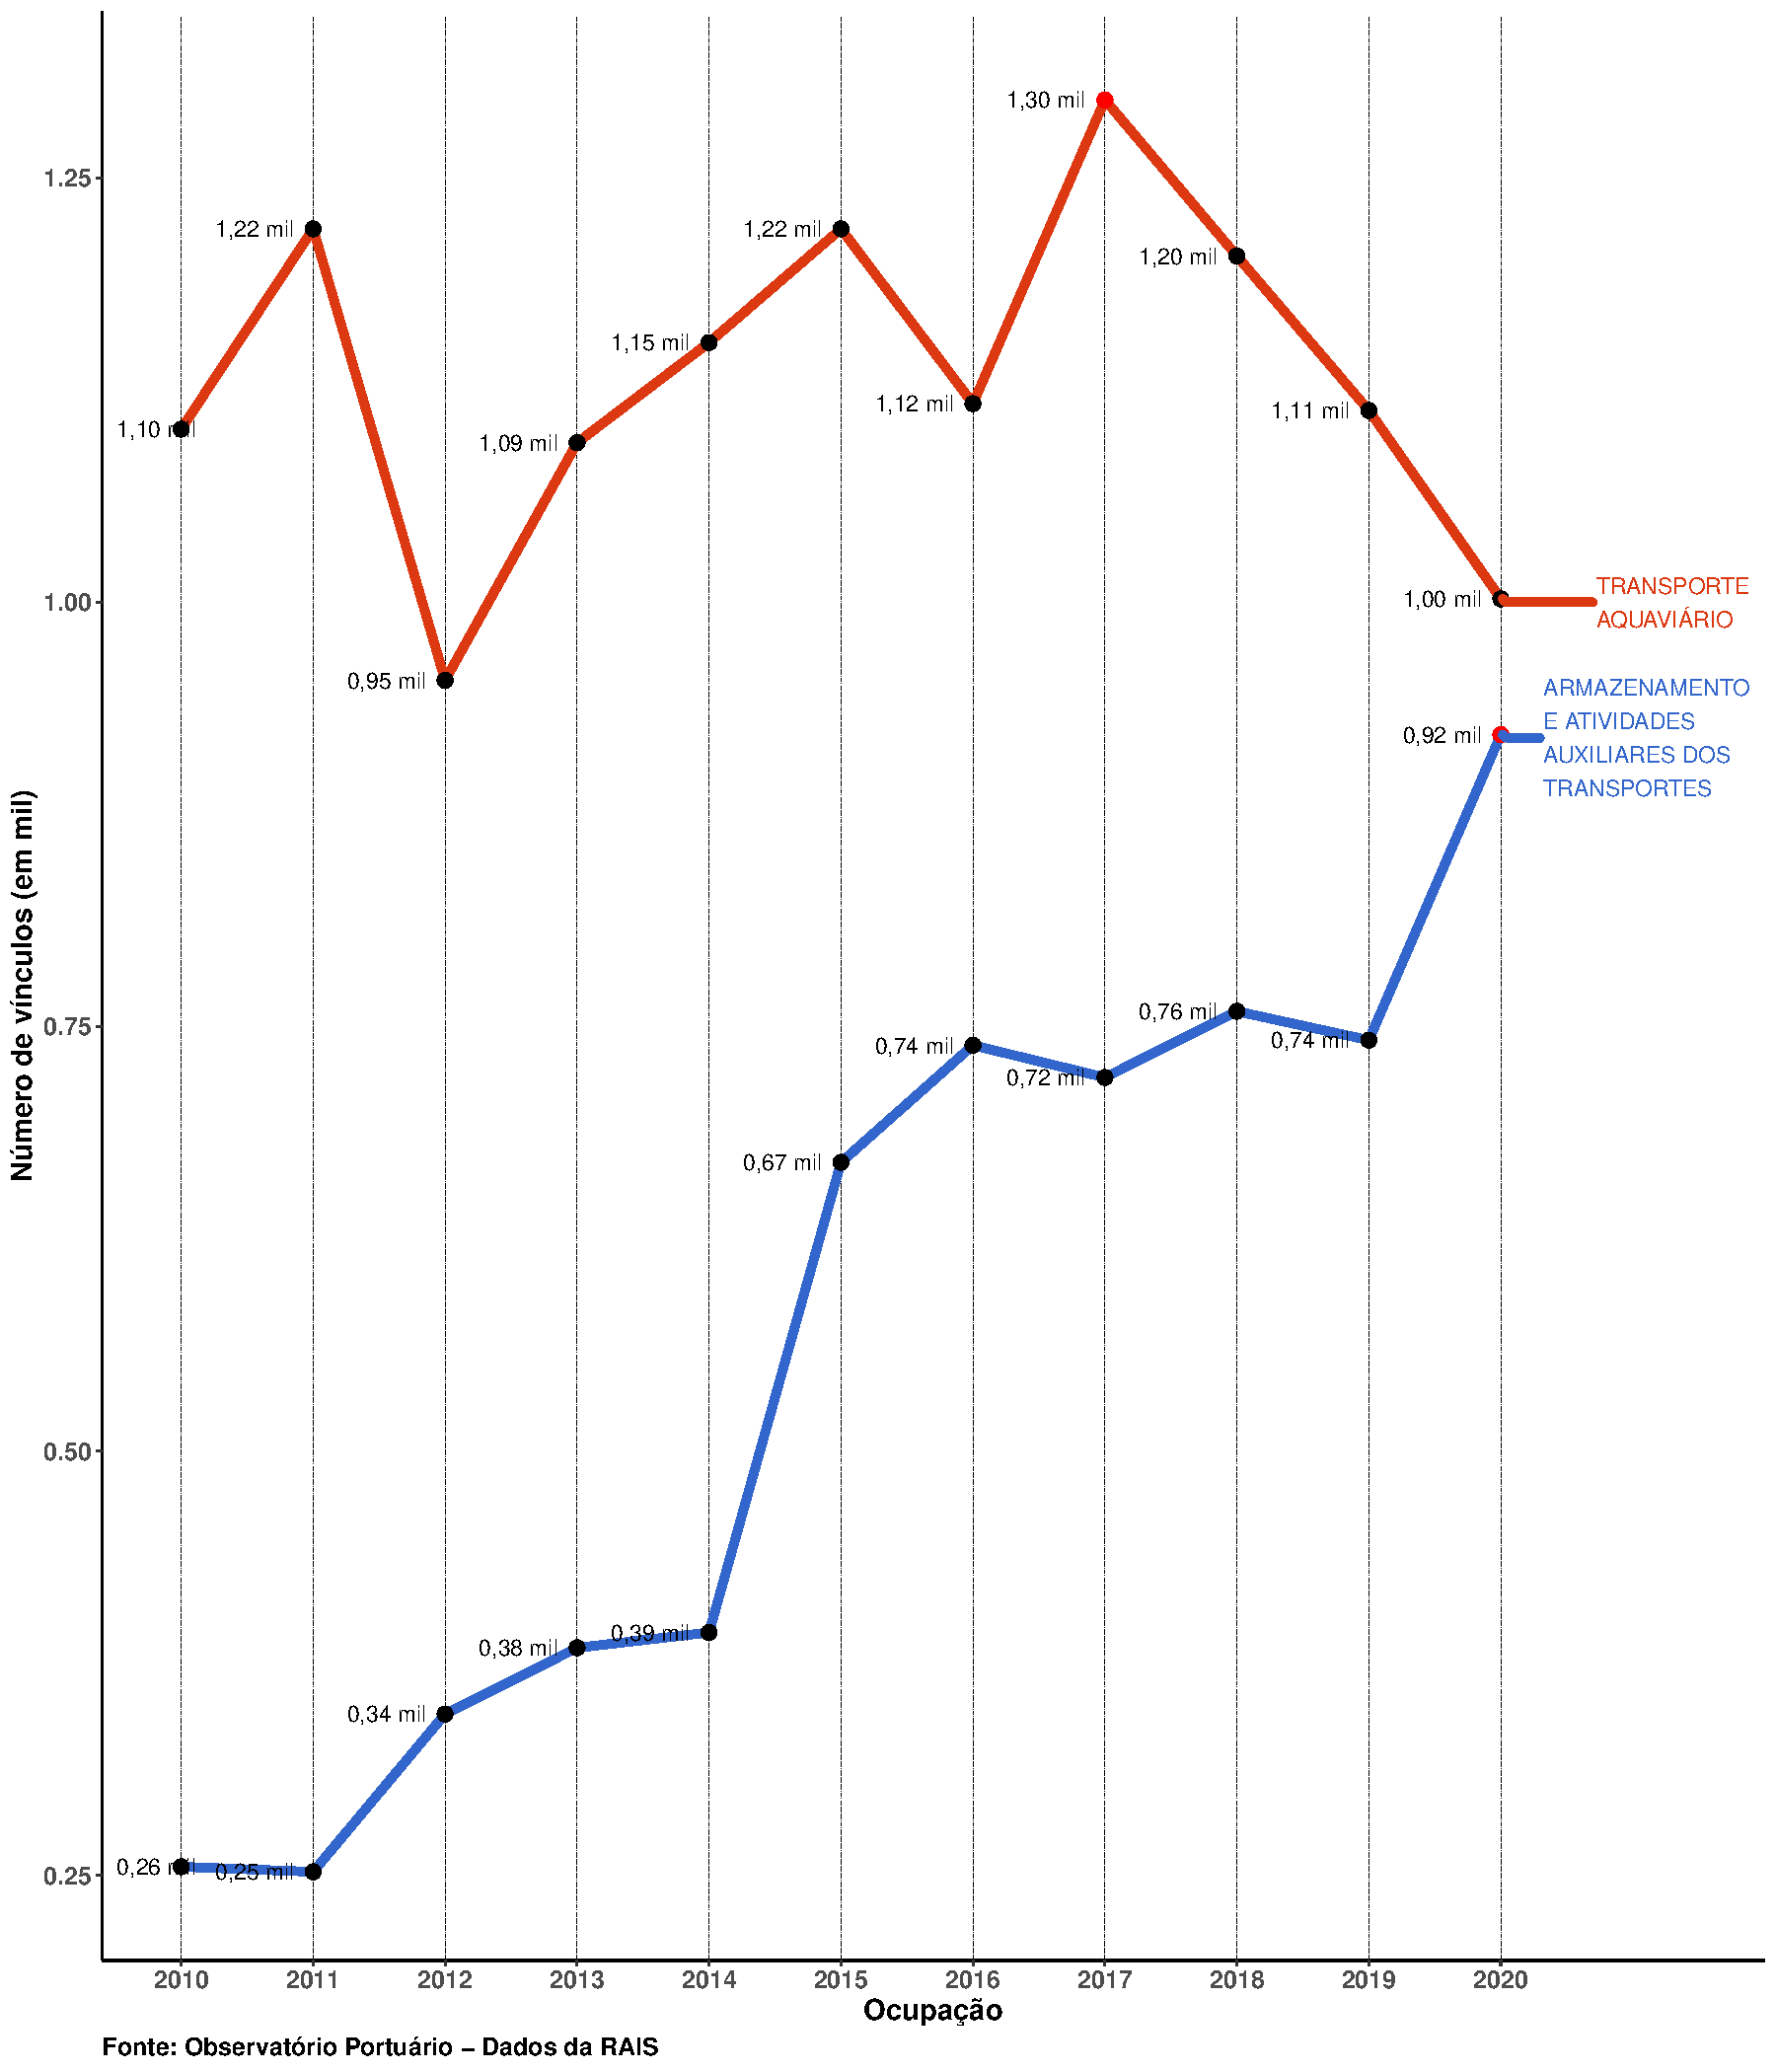
\includegraphics{mercado_trabalho_files/figure-latex/g_divisao_ma-1.pdf}

\end{document}
